% CAPÍTULO 2: FUNDAMENTAÇÃO TEÓRICA
%   DEVE SER UM CAPÍTULO ENXUTO (LEAN)
%1. Elabore um parágrafo que introduz o capítulo: Este capítulo apresenta (descreva o objetivo do capítulo...). É constituído de N seções a saber...
%2. Desenvolvimento do capítulo: os conteúdos devem ser somente os necessários para o leitor entender a sua contribuição.
%3. Trabalhos relacionados: a última seção do Capítulo 2 deve apresentar o posicionamento da sua contribuição em relação à literatura. É um detalhamento da Justificativa apresentada na Introdução.
%4. Elabore um parágrafo que conclui o capítulo e introduz o capítulo seguinte.

The proposal of this work combines the concepts of co-design and virtual reality with techniques from of Human Factors. 

In order to facilitate the understanding of this dissertation, this chapter introduces these concepts and techniques. It starts with the definition of Human Factors, also known as Ergonomics. It describes mental workload and situation awareness, as well as the corresponding assessment techniques used in this work. It then presents the concept of extended reality and defines virtual reality. Finally, it introduces the principles of co-design.

\section{Human Factor or Ergonomics}
\label{sec:human_factors}

    Studies in the area of Human Factors started during the Second World War, motivated by performance shortfalls and failures related to the operation of equipments used by humans. The studies showed that these problems could diminish when, other than engineering, psychology and physiology were also considered when designing systems that would be handled by human beings \cite{sandom2004human}.

This study area was named "Human Factors" in the United States and "Ergonomics" in Europe. Despite this difference in the names, today they are considered the same field of study. The International Ergonomics Association (IEA) defines Human Factors, therefore Ergonomics, as the following:

\begin{quote}
    \textit{"Ergonomics (or human factors) is the scientific discipline concerned with the understanding of interactions among humans and other elements of a system, and the profession that applies theory, principles, data and methods to design in order to optimize human well-being and overall system performance. Human Factors professionals contribute to the design and evaluation of tasks, jobs, products, environments and systems in order to make them compatible with the needs, abilities and limitations of people"} \cite{karwowski2012discipline}.
\end{quote}

This definition shows that humans and their interaction with systems and devices should be considered during the design process \cite{sandom2004human, sanders1998human, dul2003ergonomics}. This need resulted in the proposal of an ISO Standard: BS EN ISO 13407 "Human-centred design processes for interactive systems". It is essencial to highlight that human-centered design does not mean that the product is designed specifically for an individual. The design has to be suited to everyone, i.e., anyone that may interact with the system \cite{dul2003ergonomics}.

The interaction between humans and machines can be abstracted as illustrated in Figure \ref{fig:human_machine_representaion}. The machine receives inputs from its environment and provides information to the human operator through displays and other monitoring devices. The operator perceives the available information, process it and decides on his/her control actions. Based on the environment's inputs and operator's commands, the machine defines its outputs to the environment.

\begin{figure}[!htb]
    \centering

    \tikzstyle{arrow} = [rounded corners, line width = 1mm, bend left = 15, ->]
    
    \resizebox{0.85\width}{!}{
    \begin{tikzpicture}[node distance=1cm]
        
        \node (information) {
\includegraphics[width=.15\textwidth]{Fundamentação/Fatores Humanos/thinking.png}} 
        node(t_information)[below of = information,yshift=-0.75cm] {Information}
        node(t_information2)[below of = t_information,yshift=0.25cm] {processing};
        
        \node (controlling) [right of=information, xshift=5cm, yshift=-3cm] {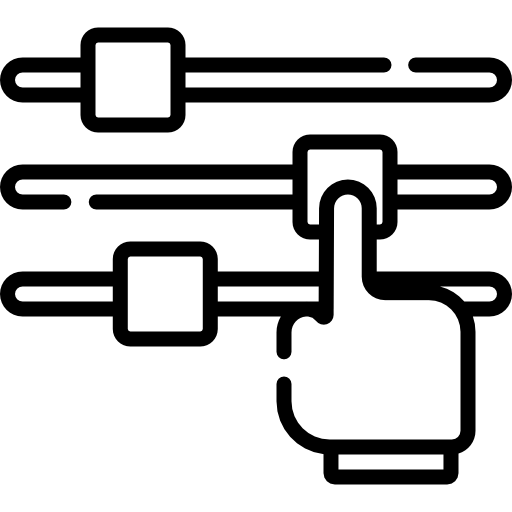
\includegraphics[width=.15\textwidth]{Fundamentação/Fatores Humanos/slider.png}}
        node(t_controlling)[below of = controlling,yshift = -0.75cm] {Controlling};
        
        \node (controls) [below of=controlling, yshift=-5cm,] {
\includegraphics[width=.15\textwidth,angle=90,origin=c]{Fundamentação/Fatores Humanos/control.png}} 
        node(t_controls) [below of = controls, yshift = -0.75cm]{Controls};
        
        \node (machine) [left of=controls, xshift=-5cm, yshift=-2cm] {
\includegraphics[width=.15\textwidth]{Fundamentação/Fatores Humanos/machine.png}} 
        node(t_machine) [below of = machine, yshift = -0.75cm]{Operation};
        
        \node (display) [left of=machine, xshift=-5cm, yshift=2cm] {
\includegraphics[width=.15\textwidth]{Fundamentação/Fatores Humanos/monitor.png}} 
        node(t_display) [below of = display, yshift = -0.75cm]{Display};
        
        \node (senses) [left of=information, xshift=-5cm, yshift=-2cm,] {\begin{tikzpicture}[node distance=1cm]
    \centering
    
    \node (eye) {
\includegraphics[width=.075\textwidth]{Fundamentação/Fatores Humanos/eye.png}};
    
    \node (ear) [right of=eye, yshift=-0.65cm] {
\includegraphics[width=.075\textwidth]{Fundamentação/Fatores Humanos/ear.png}};
    
    \node (nose) [left of=ear, yshift=-0.65cm] {
\includegraphics[width=.075\textwidth]{Fundamentação/Fatores Humanos/nose.png}};
    
    \node (hand) [right of=nose, yshift=-0.85cm] {
\includegraphics[width=.075\textwidth]{Fundamentação/Fatores Humanos/hand.png}};

\end{tikzpicture}} 
        node(t_senses) [below of = senses, yshift = -1.25cm]{Senses};
        
        \node (human) [below of=information, yshift=-4.75cm] {\Large{Human}};
        \node (human) [above of=machine, yshift=3.25cm] {\Large{Machine}};
        \node (human) [above of=information, yshift=1cm] {\Large{Work Environment}};
        
        \node (left_point) [left of=display, xshift=-2, yshift=2.75cm] {};
        \node (right_point) [right of=left_point, xshift=14cm] {};
        
        \node (input) [left of=machine, xshift=-5cm, yshift=-2cm] {\Large{Input}};
        \node (output) [right of=machine, xshift=5cm, yshift=-2cm] {\Large{Output}};
        
    
        \draw [arrow] (information.east) to (controlling.north west);
        \draw [arrow] (t_controlling.south) to (controls.north);
        \draw [arrow] (controls.west) to (machine.east);
        \draw [arrow] (machine.west) to (display.east);
        \draw [arrow] (display.north) to (t_senses.south);
        \draw [arrow] (senses.east) to (information.west);
        \draw [arrow] (input.east) -- (machine);
        \draw [arrow] (machine) -- (output.west);
        \draw [dashed,gray] (left_point) to (right_point);
        
        \draw (-8,-14) rectangle(8cm,1.5cm);
        
    \end{tikzpicture}
    }
    \caption{Human-Machine system representation. Adapted from \cite{sanders1998human}.}
    \label{fig:human_machine_representaion}
\end{figure}

Humans handle devices, machines and equipment during their daily activities. All of these manipulations are susceptible to accidents or failures that can happen because of the interaction between operator, equipment and environment. Each interface with the operator can be a factor. For example:

\begin{itemize}
    \item The operator's body position during an activity: the position can impact the operator's comfort and concentration throughout the activity, therefore, impacting the success rate or the chance of some accident happening  \cite{sanders1998human}.
    
    \item The environment's lighting: illumination can make details more noticeable without provoking discomfort or distraction and even increase productivity  \cite{sanders1998human}.
    
    \item The information displayed and manipulation of the device: the way a information is displayed on a screen, figure or text impacts how efficiently it will be understood by the operator. If this takes too long, it can draw the operator's attention for too long and compromise his/her reaction time.
    
\end{itemize}

Among the various human factors related to human-machine interaction, this work considers mental workload and situation awareness, which are explained in detail in the following sections.

\subsection{Mental Workload (MWL)}
\label{sec:mental_workload}

    Mental workload is one of the main concepts studied in Human Factors \cite{stanton2004handbook}.

In order to explain it, \citeonline{stanton2004handbook} propose an analogy with the concept of physical workload. When an athlete must lift a dumbbell (one of those gym weights bars), the strength demand from the athlete is proportional to the dumbbell's mass being lifted. If the dumbbell is lighter than the athlete's capability, it is easy enough for him to lift it. If the athlete is strong enough to carry the dumbbell, he does not feel a physical demand bigger than his capabilities. In this case, the physical workload of this activity is appropriately fitted for this athlete. Two things can happen if the dumbbell is heavier than the athlete's capability. Either the athlete adapts to lift the dumbbell using tools (adjust the strategy), or the dumbbell is not lifted completely (performance degrades). This situation corresponds to the case of a operator executing a task, which is not fitted for his capabilities.

The mental workload is similar to the physical workload but refers to the mental capacity necessary to perform a task. Each human being has a finite mental capacity. When the mental demand is higher than the operator's capacity, the person needs to adapt to finish the task, or the overall performance of the task is compromised. Otherwise, if the mental workload is too low, the operator may get bored and easily distracted and could also fail or not process the task's information.

It is important to say that mental workload is unique within each individual. It is influenced by the operator perception and also by other factors outside the task itself. These factor can be more related to the operator (like its skill, age, education, training) or the environment (like noise, heat and toxicity)  \cite{cain2007review, fallahi2016effects, cardoso2012evaluation}.

The mental workload is not a quantitative resource or something that one can directly measure, but several different techniques have been proposed in the literature to infer it. Figure \ref{fig:mwl_overview} illustrates three different classes of techniques used to evaluate mental workload explained bellow: techniques based on task performance, techniques based on physiological measures and techniques based on subjective questionnaires.
        
    \begin{figure}[!htb]
    \centering

    \tikzstyle{arrow} = [rounded corners, line width = 1mm, ->]
    
    \resizebox{0.85\width}{!}{
    \begin{tikzpicture}[node distance=1cm]
        
        \node (mwl) {
\includegraphics[width=.15\textwidth]{Fundamentação/Carga Mental/mwl.png}}
        node(t_mwl)[below of = mwl,yshift=-0.75cm] {Mental}
        node(t_mwl2)[below of = t_mwl,yshift=0.5cm] {workload};
        
        \node (demand) [above of=mwl, xshift=3cm, yshift=2.5cm] {\begin{tikzpicture}[node distance=1cm]
    \centering
    
    \node (worker) {
\includegraphics[width=.15\textwidth]{Fundamentação/Carga Mental/work.png}};
    
    \node (energy1) [above of = worker, xshift = 0.5cm, yshift = 0.05cm]
     {
\includegraphics[width=.060\textwidth]{Fundamentação/Carga Mental/bolt.png}} 
    node(energy2) [right of=energy1, xshift=-0.5cm, yshift = 0.3cm] {
\includegraphics[width=.060\textwidth]{Fundamentação/Carga Mental/bolt.png}}
    node(energy3) [left of = energy1, xshift=0.5cm, yshift = 0.3cm] {
\includegraphics[width=.060\textwidth]{Fundamentação/Carga Mental/bolt.png}};;
    
\end{tikzpicture}}
        node(t_demand)[below of = demand,yshift=-0.75cm] {Task}
        node(t_demand2)[below of = t_demand,yshift=0.5cm] {Demand};
        
        \node (capacity) [above of=mwl, xshift=-3cm, yshift=2.5cm] {
\includegraphics[width=.15\textwidth]{Fundamentação/Carga Mental/full-battery.png}}
        node(t_capacity)[below of = capacity,yshift=-0.75cm] {Mental}
        node(t_capacity2)[below of = t_capacity,yshift=0.5cm] {Capacity};
        
        \node (tasks) [left of=mwl, xshift=-4cm, yshift=-6cm] {
\includegraphics[width=.15\textwidth]{Fundamentação/Carga Mental/multitasking.png}}
        node(t_tasks)[below of = tasks,yshift = -0.75cm] {Primary and} 
        node(t_tasks2)[below of = t_tasks,yshift = 0.5cm] {secondary tasks};
        
        \node (physiological) [below of=mwl, yshift=-5cm,] {
\includegraphics[width=.15\textwidth]{Fundamentação/Carga Mental/physiological.png}} 
        node(t_physiological) [below of = physiological, yshift = -0.75cm]{Physiological}
        node(t_physiological2) [below of = t_physiological, yshift = 0.5cm]{measurements};
        
        \node (subjective) [right of=mwl, xshift=4cm, yshift=-6cm] {
\includegraphics[width=.15\textwidth]{Fundamentação/Carga Mental/subjective.png}}
        node(t_subjective) [below of = subjective, yshift = -0.75cm]{Subjective} 
        node(t_subjective2) [below of = t_subjective, yshift = 0.5cm]{measurements};
    
    
        \draw [arrow] (t_mwl2.south) to ++(0,-0.75) to +(-5,0) to (tasks.north);
        \draw [arrow] (t_mwl2.south) to (physiological.north);
        \draw [arrow] (t_mwl2.south) to ++(0,-0.75) to +(5,0) to (subjective.north);
        \draw [arrow, sharp corners] (capacity.east) to +(1.6,0) to (mwl.north);
        \draw [arrow, sharp corners] (demand.west) -- +(-1.35,0) to (mwl.north);
    
        
    \end{tikzpicture}
    }
    \caption{A overview of mental workload and the techniques to infer it.}
    \label{fig:mwl_overview}
\end{figure}    
    
    \subsubsection*{Techniques based on task performance}
    %\label{subsec:task_performance}
    
        If the mental workload influences the task performance, it would be possible to infer it using the performance's variation of a task. Because there are cases where the user's mental capacity is too high for only one task, a common approach is to add a secondary task. In this case, the user is asked to maintain a good performance level and still try to execute both tasks. Both tasks should use the same skills \cite{stanton2004handbook, sanders1998human}.
        
        For example, an experiment to assess mental workload in a flight simulator may use two tasks. The primary task is to fly the aircraft while maintaining a performance level. The second is something simple, like mentally summing two random numbers that appear on the screen. If the numbers' sum is odd, the pilot should press the left arrow key on the keyboard, otherwise should press the right arrow key. If the pilot's performance in the secondary task is too low, it means that the mental demand from the first task is too high to pay attention to the second task \cite{mohanavelu2020cognitive}.
        
%    \item Physiological measures;
    \subsubsection*{Techniques based on physiological measurements}
    %\label{subsec:physiological_measures}
    
        Many physiological measurements can be used to assess mental workload. The most common ones are heart and brain activity \cite{chakladar2020eeg, orlandi2018measuring}, skin conductance, eye movement and pupillary contraction \cite{stanton2004handbook, rodriguez2015pupillometry}. These measurements are considered an user-unbiased assessment technique \cite{fallahi2016effects}. It is recommended to evaluate them alongside another method, as they can be influenced by unknown variables and external factors. Some techniques use heart activities, obtained from an electrocardiogram (ECG) sensor, and electrodermal activity, obtained from a galvanic skin response (GSR) sensor, as physiological measurements to assess mental workload.
                
        The electrocardiogram (ECG) is a recording of the heart's electrical activity. From it, it is possible to determine the intervals between heartbeats and the corresponding frequency (heart rate, HR). Another common variable is the heart rate standard deviation (heart rate variability, HRV) \cite{cain2007review}. The heart activity is controlled by the sympathetic and parasympathetic nervous systems \cite{stanton2004handbook}. During a task, the heart activity changes with the mental demand of the task. The heart rate is expected to increase with the mental workload, while the heart rate variability is expected to decrease. These are consequences of two reactions in our system when in a mental demand situation \cite{stanton2004handbook}: a decrease in the parasympathetic nervous system activity and an increase in sympathetic nervous system activity. The ECG is a simple and non-invasive sensor used in many experiments to evaluate mental workload and other human factors' \cite{mohanavelu2020cognitive, mansikka2016fighter, zhang2014detection}.
         %(DEFINIR MELHOR)
                
         The skin electrodermal activity is affected by the person's sweating and the level of moisture in the environment. It can be used to reveal changes in our sympathetic system \cite{nourbakhsh2012using, shi2007galvanic}. It has been used in the literature as an assessment technique for stress and arousal \cite{nourbakhsh2012using, stanton2004handbook, shi2007galvanic}, the usability of human-computer systems \cite{shi2007galvanic} and also mental workload \cite{zhang2014detection, borghini2014measuring}.
    
    \subsubsection*{Techniques based on subjective questionnaires}
    %\label{subsec:subjective_measures}    

        The use of subjective questionnaires to assess mental workload has been extensively discussed in the literature \cite{sanders1998human, stanton2004handbook}. The questionnaires can be unidimensional or multidimensional. The unidimensional questionnaires are more straightforward by provide only a general workload score.     Examples of multidimensional questionnaires are the Subjective Workload Assessment Technique (SWAT) and the NASA Task Load Index (NASA-TLX). SWAT decomposes the mental in three dimensions: time load, mental effort load, and psychological stress. NASA-TLX, a questionnaire created by \citeonline{hart1988development}, uses six dimensions, as described in Table \ref{tab:nasa_dimensions}. These questionnaires were proposed to evaluate only one task/activity. If the user has performed two tasks (a primary and secondary task), he/she should be oriented to answer about the primary task, not a combination of both \cite{sanders1998human}.
        
        \begin{table}[htb]
            \centering
            \caption{NASA-TLX dimensions and the description of each dimension. \cite{stanton2004handbook}.}
            \label{tab:nasa_dimensions}
                \begin{tabular}{|l|l|}

                    \hline
                    \textbf{Dimension}   & \textbf{Explanation}                                                                                                                                                   \\ \hline
                    Mental demand (MD)   & \begin{tabular}[c]{@{}l@{}}The mental and perceptive activity\\ demanded by the task (chose, decide,\\ think, calculate, search, etc.).\end{tabular}                       \\ \hline
                    Physical demand (PD) & \begin{tabular}[c]{@{}l@{}}The physical activity demanded by\\ the task (pull, lift, spin, drag, etc.).\end{tabular}                                                       \\ \hline
                    Temporal demand (TD) & \begin{tabular}[c]{@{}l@{}}The time pressure felt by the user.\\ A rating the leverages the time \\ available and the time necessary to\\ completed the task.\end{tabular} \\ \hline
                    Performance (PE)     & \begin{tabular}[c]{@{}l@{}}The user's satisfaction with its \\ performance or result the task.\end{tabular}                                                                \\ \hline
                    Effort (EF)          & \begin{tabular}[c]{@{}l@{}}A rating of the effort necessary \\ to achieve that performance felt by\\ the user.\end{tabular}                                                 \\ \hline
                    Frustration (FR)     & \begin{tabular}[c]{@{}l@{}}A rating of stress, annoy or irritation\\ felt by the user throughout the task.\end{tabular}                                                    \\ \hline
                \end{tabular}
        \end{table}
            
        Finally, it is essential to highlight that, to have a comprehensive evaluation of the mental workload, not to choose only one technique, but to combine techniques from the three classes (task performance, physiological measurements and subjective questionnaires). Mental workload is multidimensional and can reflect partially or differently in each technique \cite{sanders1998human}.

\subsection{Situation Awareness (SA)}
\label{sec:situation_awareness}

    Situation awareness can be defined as “the perception of the elements within a volume of time and space (Level 1), the comprehension of their meaning (Level 2), and the projection of their status in the near future (Level 3)” as illustrated in Figure \ref{fig:sa_overview}. One example is when an air traffic controller looks at a radar display (Level 1). He/she seeks to understand the aircraft's position and speed (Level 2) and then predict its position in the near future, 5, 10 or 15 minutes after (Level 3) \cite{sanders1998human}. Similarly, when a pilot reads the cockpit panel (Level 1) and understands their data (Level 2) then he/she can predict the next reading of that same instrument or some other status of the aircraft after a couple of minutes (Level 3).

\begin{figure}[!htb]
    \centering
    \tikzstyle{arrow} = [rounded corners, line width = 1mm, ->]

    \resizebox{0.85\textwidth}{!}{
    \begin{tikzpicture}[node distance=3.3cm]
        \centering
        
        \node (info) [fill=white] {
\includegraphics[width = 0.20\textwidth]{Fundamentação/Percepção situacional/information.png}}
        node(t_info)[below of = info,yshift=1.3cm] {\Large Information};
        
        \node (arrow) [right of=info, xshift=7.0cm, yshift = -0.5cm] {\begin{tikzpicture}[node distance=5cm, line width = 2.5mm]
    \centering

    \node (seta1) [] {};
    \node (seta2) [right of = seta1, xshift = 5.0cm] {};
    \node (seta3) [above of = seta2, yshift = -2.5cm] {};
    \node (seta5) [below of = seta1, yshift = -1.5cm,] {};
    \node (seta6) [right of = seta5, xshift = 5.0cm] {};
    \node (seta7) [below of = seta6, yshift = 2.5cm] {};
    \node (seta4) [right of = seta1, below of = seta1, yshift = 1.75cm, xshift = 10.0cm] {};

    \draw (seta1.center) -- (seta2.center);
    \draw (seta2.center) -- (seta3.center);
    \draw (seta3.center) -- (seta4.center);
    \draw (seta4.center) -- (seta7.center);
    \draw (seta7.center) -- (seta6.center);
    \draw (seta6.center) -- (seta5.center);
    \draw (seta5.center) -- (seta1.center);
    

\end{tikzpicture}
};
        
        \node (perception) [right of=info, xshift=2.5cm, draw, line width=2mm] {\begin{tikzpicture}[node distance=5cm]
    \centering
    
    \node (comprehension) {
\includegraphics[width=3.0cm]{Fundamentação/Percepção situacional/eye.png}};

    \node(info) [] {
\includegraphics[width=1.0cm]{Fundamentação/Percepção situacional/information}};

\end{tikzpicture}}
        node(t_perception)[below of = perception, yshift=0.9cm] {\Large 1st Level}
        node(t_perception2)[below of = t_perception, yshift=2.5cm] {\Large Perception};

        \node (comprehension) [right of=perception, xshift=0.25cm, draw, line width=2mm] {\begin{tikzpicture}
    \centering
    
    \node (comprehension) {
\includegraphics[width=3.0cm]{Fundamentação/Percepção situacional/idea.png}};
    
    \node(info) [yshift = 0.5cm] {
\includegraphics[width=0.75cm]{Fundamentação/Percepção situacional/information}};

\end{tikzpicture}}
        node(t_comprehension)[below of = comprehension, yshift=0.9cm] {\Large 2nd Level}
        node(t_comprehension2)[below of = t_comprehension, yshift=2.5cm] {\Large Comprehension};

        \node (projection) [right of=perception, xshift=3.75cm, draw, line width=2mm] {\begin{tikzpicture}[node distance=5cm]
    \centering
    
    \node (comprehension) {
\includegraphics[width=3.0cm]{Fundamentação/Percepção situacional/future.png}};

    \node(info) {
\includegraphics[width=1.5cm]{Fundamentação/Percepção situacional/information}};

\end{tikzpicture}
}
        node(t_projection)[below of = projection, yshift=0.9cm] {\Large 3rd Level}
        node(t_projection2)[below of = t_projection, yshift=2.5cm] {\Large Projection};

        \node (decision) [right of=projection, xshift=5.0cm] {
\includegraphics[width = 0.30\textwidth]{Fundamentação/Percepção situacional/decision.png}}
        node(t_decision)[below of = decision, yshift=0.5cm] {\Large Decision}
        node(t_decision2)[below of = t_decision, yshift=2.5cm] {\Large making};

    \end{tikzpicture}
    }
    \caption{An overview of situation awareness and the SAGAT.} %and the methods to infer it
    \label{fig:sa_overview}
\end{figure}

The term “situation awareness” was first proposed for the Aeronautics domain and today is considered a key factor for designing complex and dynamic systems from other domains, such as automotive, medical and nuclear \cite{endsley1995measurement}. It is an essencial factor to make sure that the user will be capable to make important decisions correctly and achieve high-performance \cite{endsley1988design, endsley2018automation}.

As it is for the mental workload, situation awareness is not a quantitative subject. The most common way to measure it is using subjective techniques, among which one of the most famous is the Situation Awareness Global Assessment Technique (SAGAT). It was proposed by \cite{endsley1988design} and is based on how the information is processed inside the user’s mind. The test application is made by freezing the operator activity, usually made in a simulation environment, and then asking the user some questions that were previously defined based on the user's activity. These questions should be as similar as possible to how the person thinks when reasoning about the situation to avoid extra effort in understanding it \cite{stanton2004handbook}.  Although freezing the activity may sound troublesome, empirical work has shown that it does not interfere with the user performance and the user memory can withstand a break for as long as 5 to 6 min \cite{endsley1988design}.


\section{Extended Reality (XR)}
\label{sec:extended_reality}

    Extended reality is a broad term that refers to all different ways of combining virtual and real entities in a human-machine interface system. It is usually decomposed into four classes (augmented reality, augmented virtuality, mixed reality, and virtual reality) that differ on the level of reality and virtuality involved in the interface system. 

\citeonline{milgram1994taxonomy} organized these classes and created the concept of the “virtuality continuum”, as illustrated in Figure, as illustrated in Figure \ref{fig:virtuality_continuum}. On the extreme left, the real environment represents the cases where the user operates physical elements inside that environment. Along the path to the right, the environment starts to incorporate digital elements until it reaches the far right, where all the elements in the environment are virtual and have a digital origin \cite{nijholt2005virtuality, doolani2020review}. The first step from the "Real Environment" to "Virtual Reality" is the augmented reality.

\begin{figure}[!htb]
    \tikzstyle{arrow} = [ccmDBlue, rounded corners, line width = 2mm, ->]
    \tikzstyle{--blue} = [ccmDBlue, rounded corners, line width = 2mm]
    \tikzstyle{--black} = [rounded corners, line width = 1mm]
    
    %\tikzstyle{arrow_flow} = [ccmblue, rounded corners, line width = 2mm, ->]
    %\tikzstyle{arrow_return} = [ccmred, rounded corners, line width = 2mm, ->]
    
    \resizebox{0.80\width}{!}{
    \begin{tikzpicture}[node distance=1cm]
        \centering
    
        \node (left) {};
        
        \node (reality) [right of = left, xshift = 2cm]{
\includegraphics[width=.15\textwidth]{Fundamentação/Realidade Extendida/real.png}}
        node(t_reality)[below of = reality,yshift=-0.75cm] {Real}
        node(t_reality2)[below of = t_reality,yshift=0.5cm] {Environment};
        
        \node (midLeft) [right of = reality, xshift = 1cm] {};
        
        \node (ar) [right of=reality, xshift=3cm] {
\includegraphics[width=.15\textwidth]{Fundamentação/Realidade Extendida/ar.png}}
        node(t_ar)[below of = ar,yshift=-0.75cm] {Augmented}
        node(t_ar2)[below of = t_ar,yshift=0.5cm] {Reality};
        
        \node (av) [right of=ar, xshift=3cm] {
\includegraphics[width=.15\textwidth]{Fundamentação/Realidade Extendida/av.png}}
        node(t_av)[below of = av,yshift=-0.75cm] {Augmented}
        node(t_av2)[below of = t_av,yshift=0.5cm] {Virtuality};
        
        \node (vr) [right of=av, xshift=3cm] {
\includegraphics[width=.15\textwidth]{Fundamentação/Realidade Extendida/vr.png}}
        node(t_vr)[below of = vr,yshift = -0.75cm] {Virtual} 
        node(t_vr2)[below of = t_vr,yshift = 0.5cm] {Reality};
        
        \node (midRight) [left of = vr, xshift = -1cm] {};
        
        \node (right) [right of = vr, xshift = 2cm] {};
        
        \node (mr) [above of=ar, right of=ar, xshift=1cm, yshift=3cm] {
\includegraphics[width=.15\textwidth]{Fundamentação/Realidade Extendida/mr.png}} 
        node(t_mr) [below of = mr, yshift = -0.50cm]{Mixed}
        node(t_mr2) [below of = t_mr, yshift = 0.5cm]{Reality};
        
        \draw [arrow] (reality) to (left);
        \draw [--blue] (reality) to (ar);
        \draw [--blue] (ar) to (av);
        \draw [--blue] (av) to (vr);
        \draw [arrow] (vr) to (right);
        \draw [--black] (mr.west) -- +(-2.6,0) to (midLeft);
        \draw [--black] (mr.east) -- +(2.6,0) to (midRight);
         
        
        \node (left) [left of = reality, xshift = -2cm] {};
        \node (right) [right of = vr, xshift = 2cm] {};
    
        
    \end{tikzpicture}
    }
    \centering
    \caption{The Virtuality Continuum concept. Adapted from \cite{milgram1994taxonomy}}
    \label{fig:virtuality_continuum}
\end{figure}

In the augmented reality system, the user sees some digital elements that are laid over the real environment. without making the user lose his sense of presence in the real world. These elements can be text, images, video, etc. Augmented reality can be used to assist workers in manufacturing and assembly tasks, as well as training \cite{doolani2020review, farrell2018learning, ma2007virtuality}.
    
While the augmented reality brings digital elements to the real environment, the augmented virtuality creates an environment that could only exist digitally, such as a fantasy world from games or movies. This scenario is the background of some other activity that is being done by the user in the real environment. An example is to train a pilot in a virtual environment but with an accurate mock-up of the cockpit, which provides physical buttons and inceptors for the pilot to touch and hold \cite{farshid2018go}. Another example is to play sports, such as tennis, golf or baseball, in a complete digital arena but using the actual equipment with a tracker. \citeonline{kirner2012using} also add that augmented reality has three characteristics: it combines real and virtual elements; it has real time interaction; and three-dimensional.

The mixed reality stays in between the real and virtual environments. Unlike augmented reality and augmented virtuality, in a mixed reality system the user can manipulate digital elements as if they were inside the real world \cite{doolani2020review}. One example is when a client from a furniture store uses mixed reality not only to see how the furniture fits inside his room, but he can also move it and change its color, size and shape before buying or even going to the shop.
    
On the far right of the virtuality continuum, the virtual reality is when the user is the only non-digital element, everything else is digital, immersing the user in a virtual environment, but, of course, inside the physical limits of the real environment \cite{ma2007virtuality}. If the feeling of presence inside that environment is well tailored, the user can momentarily forget about the real environment and act and react accordingly to the virtual environment \cite{farrell2018learning}. 
    
Virtual reality is a powerful tool that allows a user to be transported to a tridimensional environment that could be out of reach or that does not exist but is needed for testing or training reasons \cite{mujber2004virtual}. Inside this virtual environment, the user can walk, look around and feel as if the environment was real \cite{salah2019virtual}.

Figure \ref{fig:ar_av_mr} shows the representations of each of these Extended Reality classes.

\begin{figure}[!htb]
    \tikzstyle{arrow} = [ccmblue, rounded corners, line width = 2mm, ->]
    \tikzstyle{--blue} = [ccmblue, rounded corners, line width = 2mm]
    \tikzstyle{--black} = [rounded corners, line width = 1mm]
    
    \resizebox{0.85\width}{!}{
    \begin{tikzpicture}[node distance=1cm]
        \centering
    
        \node (ar) {
\includegraphics[width=0.3\textwidth]{Fundamentação/Realidade Extendida/ar.png}}
        node(t_ar)[below of = ar,yshift=-2.0cm] {Augmented}
        node(t_ar2)[below of = t_ar,yshift=0.5cm] {Reality};
        
        \node (av) [right of=ar, xshift=5cm, yshift = 0.1cm] {
\includegraphics[width=.34\textwidth]{Fundamentação/Realidade Extendida/av.png}}
        node(t_av)[below of = av,xshift = 1.0cm, yshift=-2.0cm] {Augmented}
        node(t_av2)[below of = t_av,yshift=0.5cm] {Virtuality};
        
        \node (mr) [below of=ar, yshift=-5.5cm] {
\includegraphics[width=.31\textwidth]{Fundamentação/Realidade Extendida/mr.png}}
        node(t_mr)[below of = mr,yshift=-2.0cm] {Mixed}
        node(t_mr2)[below of = t_mr,yshift=0.5cm] {Reality};
        
        \node (vr) [right of=mr, xshift=5.0cm, yshift = -0.5cm] {
\includegraphics[width=.25\textwidth]{Fundamentação/Realidade Extendida/vr.png}}
        node(t_vr)[below of = vr,yshift = -1.5cm] {Virtual} 
        node(t_vr2)[below of = t_vr,yshift = 0.5cm] {Reality};
        
        \node (n) [right of = ar, above of = ar , xshift = 2cm, yshift = 3.0cm] {};
        \node (l) [right of = av, below of = av, xshift = 3cm, yshift = -3.1cm] {};
        \node (s) [left of = vr, below of = vr, xshift = -2cm, yshift = -3.0cm] {};
        \node (o) [left of = mr, above of = mr, xshift = -3cm, yshift = 1.6cm] {};
        
        
        %\draw [arrow] (reality) to (left);
        %\draw [--blue] (reality) to (ar);
        %\draw [--blue] (ar) to (av);
        %\draw [--blue] (av) to (vr);
        %\draw [arrow] (vr) to (right);
        \draw [--black] (n) to (s);
        \draw [--black] (l) to (o);
         
        
        %\node (left) [left of = reality, xshift = -2cm] {};
        %\node (right) [right of = vr, xshift = 2cm] {};
    
        
    \end{tikzpicture}
    }
    \centering
    \caption{A represantion of the differences between AR, AV, MR and VR. Made by the author}
    \label{fig:ar_av_mr}
\end{figure}

Although some researchers still use this classification, it is considered outdated by others. Nowadays the shift between augmented reality and augmented virtuality is not gradual because they group different styles of interaction, have different equipments necessary to create the interface and has other technologies that at the time the virtuality continuum was conceived it was not considered \cite{cerqueira2019tangible}.

For \citeonline{kirner2012using} consider an additional class: cross-reality. It is the combination of having a virtual environment and a real environment connected with sensors and actuators creating a bidirection information feed between both environments.    

\section{Co-Design}
\label{sec:co_design}

    Co-design, or collaborative design, refers to a design process in which individuals of the design team have different backgrounds or bring different experiences, which can be essencial for the product under design. It is based on good communication and information sharing among the team \cite{chiu2002organizational}.

\citeonline{kleinsmann2006understanding} provides the following definition:.

\begin{quote}
    \textit{"Collaborative design is the process in which actors from different disciplines share their knowledge about both the design process and the design content. They do that to create a shared understanding of both aspects, to be able to integrate and explore their knowledge and to achieve the larger common objective: the new product to be designed."} \cite{kleinsmann2006understanding}.
\end{quote}

This definition emphasizes two critical aspects of co-design: knowledge sharing and integration. According to \citeonline{kleinsmann2006understanding} knowledge is the data after the receiver's understanding or translating process, in a state that is possible to record or register, so that the person can remember and use it later. During the collaborative design, ideas, facts or concepts are exchanged between the actors. This exchange is a fundamental part of the co-design process since it is responsible for the growth of each individual's knowledge. Once the knowledge is shared among the actors, they can use it when performing their tasks, resulting in knowledge integration \cite{kleinsmann2006understanding}.

\section{Final remarks}
\label{sec:final_remarks2}

%Colocar um resumo do capitulo descrevendo também como os tres temas abordados são combinados no seu trabalho. Colocar uma seção de final remarks ao final de cada capitulo, com excecao do primeiro e do ultimo.

This chapter is dedicated to introducing the fundamental concepts, which are necessary for understanding the proposal of this Master's dissertation. It starts by describing the importance of Human Factors in improving human-machine interaction. Two important concepts of Human Factors are presented: mental workload and situation awareness. For each of them, the main assessment techniques are described.

Next, the concepts of extended and virtual reality are discussed, as well as other variations such as augmented reality and augmented virtuality.

Finally, the approach of co-design is proposed as a way of integrating different stakeholders into the design process. 

The next chapter discusses recently published work that are related to the proposal of this work.
